\section{OpenCL ray casters}
\label{sec:opencl_caster}

\begin{figure}
\centering
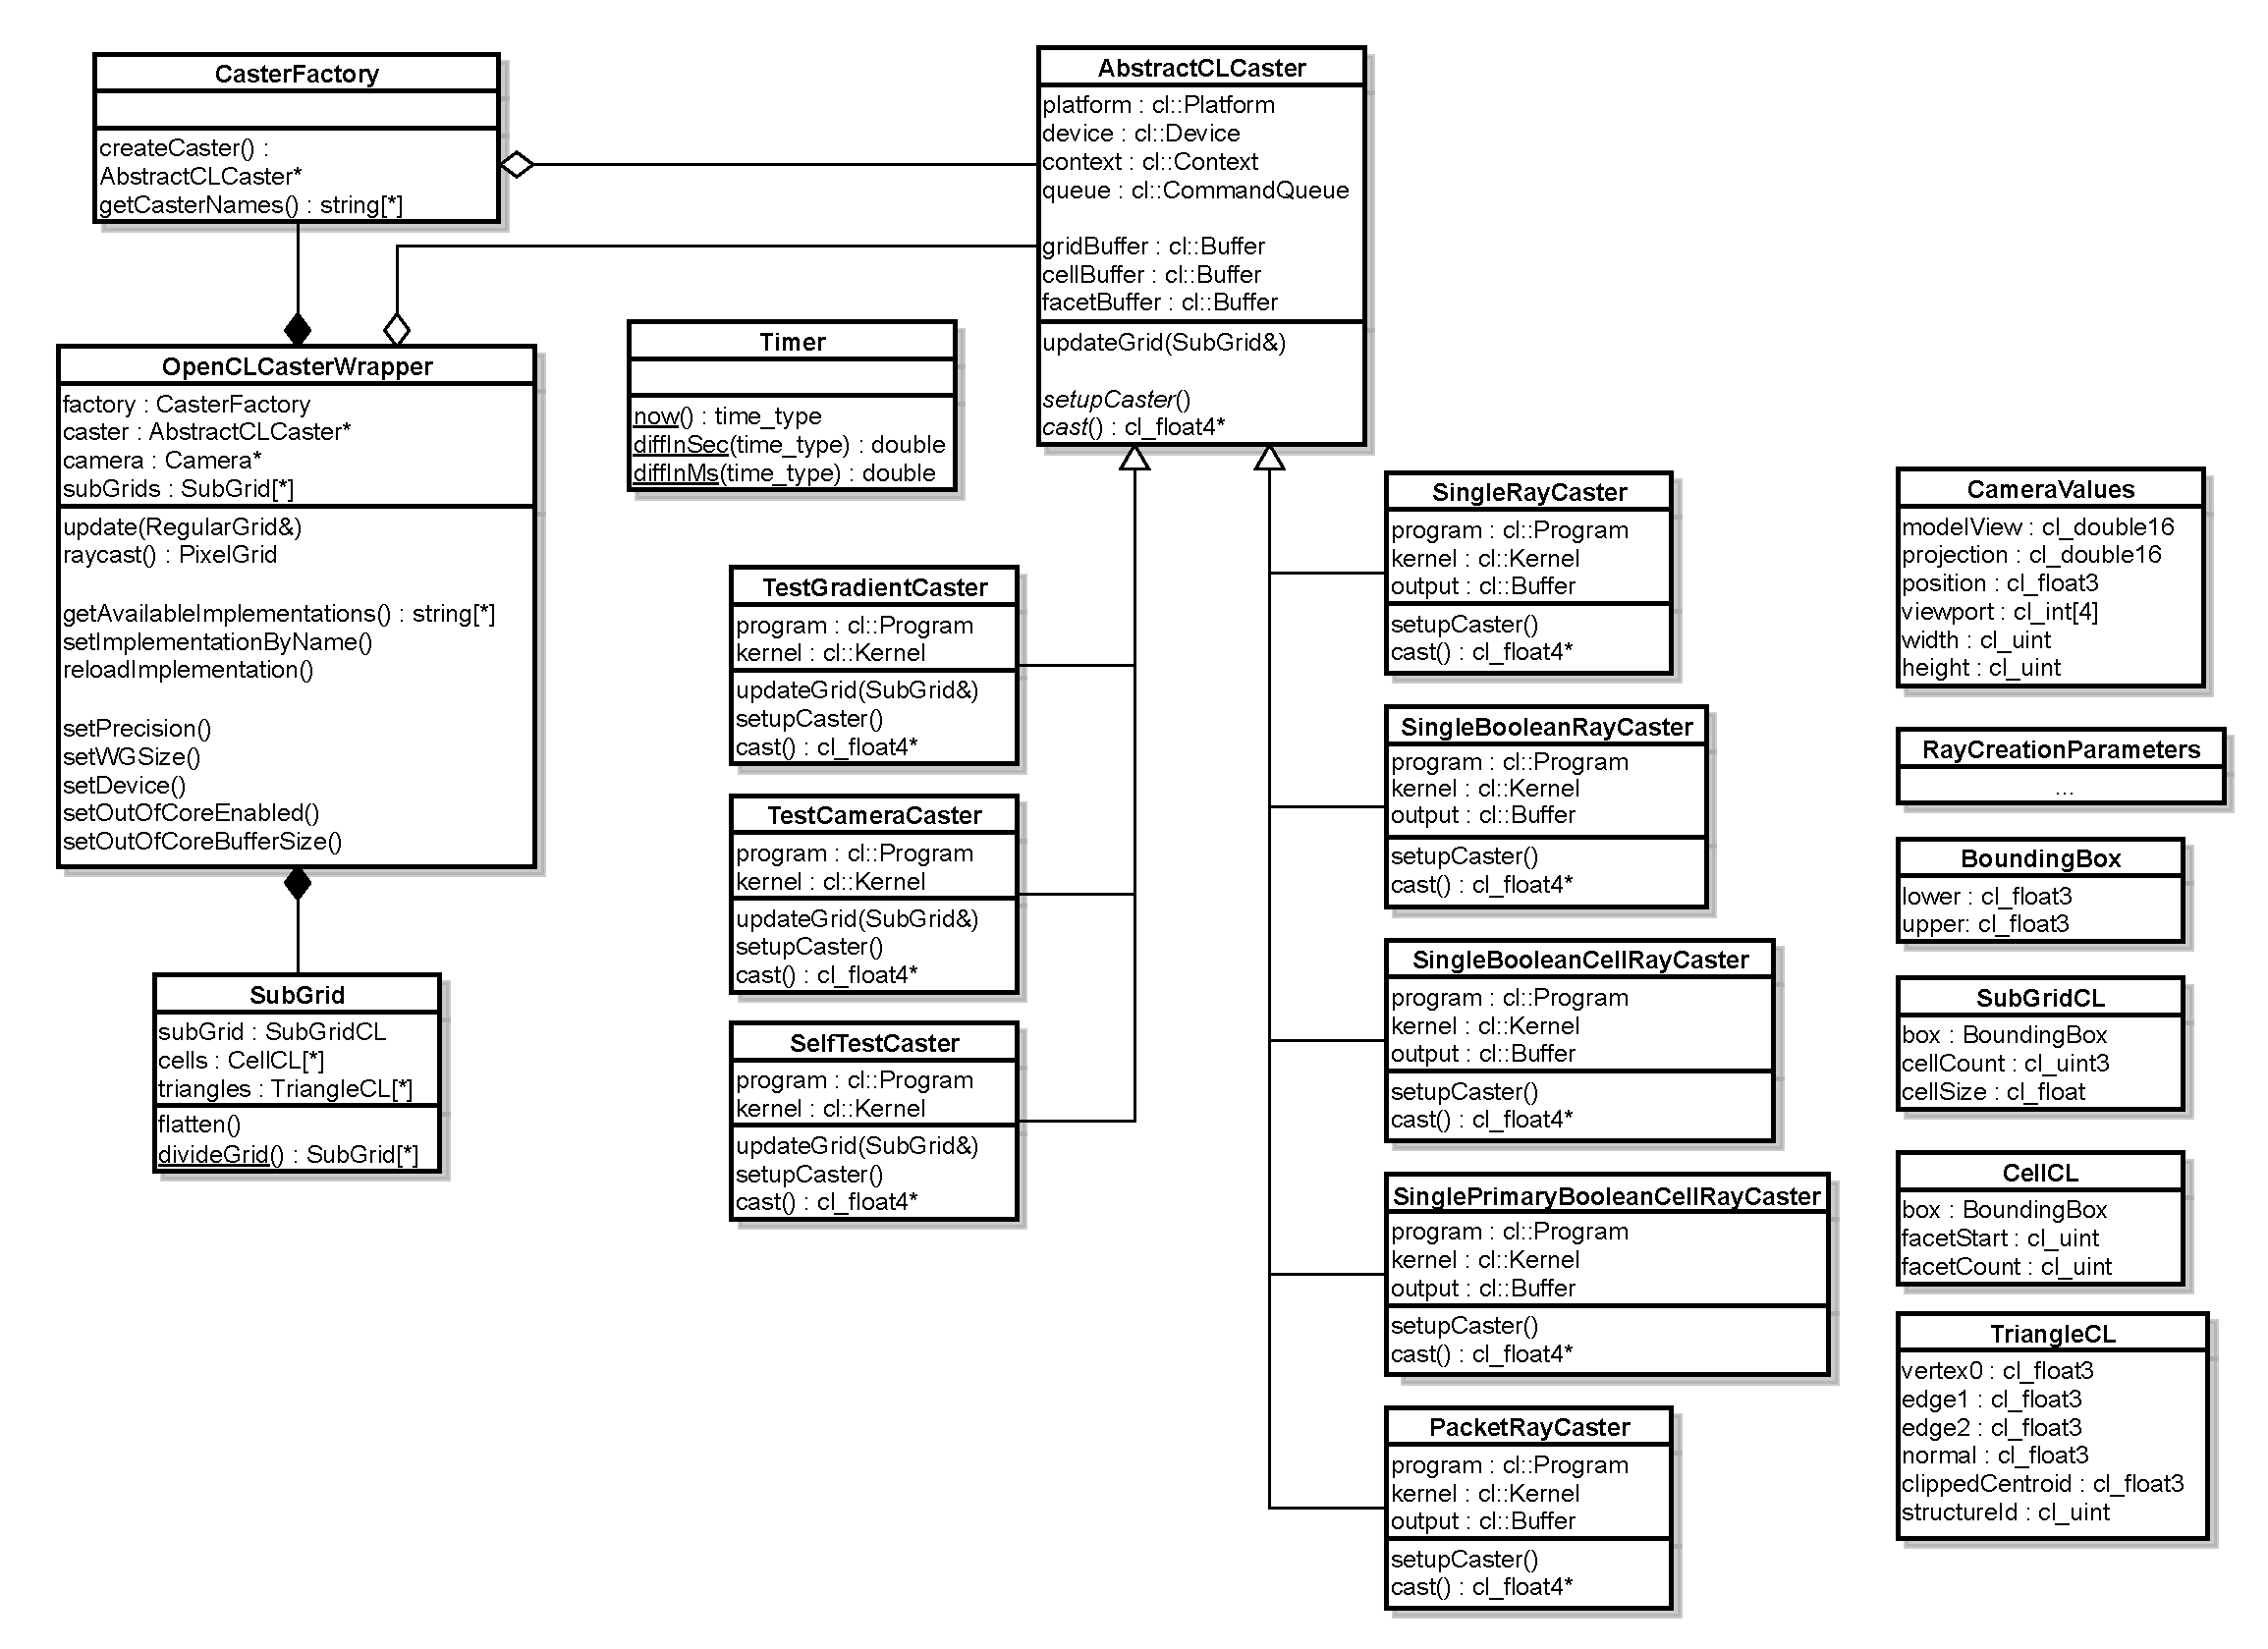
\includegraphics[width=\textwidth]{enlight_opencl_class_diagram}
\caption{Simplified class diagram of the OpenCL ray casting driver.}
\label{fig:enlight_opencl_class_diagram}
\end{figure}

\subsection{OpenCL driver}

big picture, class diagram

where does the OpenCL driver integrate into the existing prototype?

include files (do not export dependencies)

\subsection{Extensions of host application}

console commands

\subsection{TestGradientCaster}

Proof of concept, testing OpenCL functionality, enqueuing first kernel, retrieving result as image, returning image to host application for display

\subsection{TestCameraCaster}

Integration of camera position and perspective, ray factory, first ray casting attempt, grid not used yet, primitive geometry (cube) statically stored in kernel,

\subsubsection{Ray creation routines}

ray creation parameters, matrices, formulas

\subsubsection{Fast triangle intersection routine}

paper + explanation

\subsection{SelfTestCaster}

Validating host/device interaction by querying size of transfer structs and comparing them with the host's

\subsection{SingleRayCaster}

First full ray caster attempt, uses grid

\subsubsection{Data structure for grid}

flattening grid into arrays for OpenCL buffers, host/device data structures

\subsubsection{Traversing grid using 3DDDA}

explain 3DDDA

\subsection{SingleBooleanRayCaster}

does calculate all intersections inside a cell

depth-order intersections with sorting algorithm

loop over intersections and alter ray global counter

problem with intersection buffer

\subsection{SingleBooleanCellRayCaster}

reduce intersection counting to cell only

therefore, inside counter has to be determined at cell entry using secondary rays to each structure

\subsection{Double support}

via preprocessor, remain compatible with GPUs not supporting double

\subsection{OpenCL source embedding}

custom build step

convert source files to header and compile into executable

\subsection{SinglePrimaryBooleanCellRayCaster}

merging inside counter determination with intersection precalculation, secondary rays are now only created if primary ray does not hit a structure (achieves more stability)

\subsection{PacketRayCaster}

Motivation, huge performance boost on CPU, keep rays more coherent (fits GPUs hardware profile)

required changes

\subsubsection{Slice traverser}

replaces 3DDA, paper, describe algorithm

drawbacks of GPU implementation (loads of syncronizations)

\subsection{Migration to new host application}
\label{sec:migration}

removing legacy code, integrating new C++ component framework (CWC, Michael Hava)

port of OpenCL driver

\subsection{Out of core casting}

Motivation, older GPUs, large models

Changes to data structure and OpenCL driver

